% =====================================================================
% AUDIT NOTES — RUNNING LOG OF ITEMS TO ADDRESS LATER
% =====================================================================
%
% This file tracks fixes, additions, and consistency items identified
% during the chapter-by-chapter audit but deferred to when the relevant
% chapter is reached. Updated continuously as the audit progresses.
%
% Last updated: during the introduction chapter audit
% =====================================================================


% =====================================================================
% FOR conclusion.tex (CONCLUSION CHAPTER, AUDITED LAST) — DONE
% =====================================================================
%
% All conclusion-specific items resolved during the conclusion-chapter
% audit. Summary of changes applied:
%
% 1. ✓ BaldwinSivek2022 -> Binns2023 (line 33): the unique-composite-
%    almost-L-space-knot uniqueness result is from Binns, not from
%    Baldwin-Sivek.
%
% 2. ✓ "filtered chain homotopy type" -> "bigraded structure" (cosmetic
%    surgery subsection): no longer applicable since the cosmetic
%    surgery subsection was removed (see #4 below).
%
% 3. ✓ LosInfiniteSequence -> LosAlgorithm (line ~59): substantively
%    correct attribution. The "algorithmic realization" call is from
%    Los's 1993 algorithm paper, not the 2008 fixed-point-free paper.
%
% 4. ✓ Cosmetic surgery subsection REMOVED. Tao 2019 (arXiv:1909.05048)
%    established CSC for all composite knots topologically; the HFK-
%    derived corollary is not new. Same treatment as the intro.
%
% 5. ✓ Khovanov subsection EXPANDED with the BDLLS-adapted strategy
%    drafted in outlook_chapter_drafts.tex.
%
% 6. ✓ Wang family subsection ADDED after the Khovanov subsection,
%    drafted in outlook_chapter_drafts.tex.
%
% 7. ✓ "Generalizing the autofolder" second bullet sharpened: now
%    points back to Section \ref{subsec:dilatation_enumeration_intro}
%    in the introduction rather than restating the bounded-dilatation
%    application. Required adding \label{subsec:dilatation_enumeration_intro}
%    to the intro's "Enumerating Pseudo-Anosovs of Bounded Dilatation"
%    subsection.
%
% 8. ✓ Cable detection theorem statement (Theorem 11.X in summary)
%    rewritten to match the actual statement of thm:cable_detection_partial:
%    two alternatives (K is the cable, OR K is hyperbolic and falls
%    in the residual list), with the non-hyperbolic detection as a
%    "in particular" clause.


% 9. ✓ "Detection beyond genus two" subsection REVISED to include the
%    hyperelliptic-monodromy caveat. The original text claimed the
%    framework "extends in principle to higher-genus fibered knots"
%    with the obstruction being only "rapid growth in complexity of
%    the train track state space" — this understates the structural
%    issue. The corrected version states:
%      - genus 2: hyperelliptic involution is CENTRAL in Mod(Sigma_2),
%        so Mod = H (the hyperelliptic mapping class group); every
%        monodromy descends via Birman-Hilden.
%      - genus >= 3: H is a PROPER subgroup of Mod, so Birman-Hilden
%        descent applies only to "hyperelliptic" (symmetric)
%        monodromies.
%    Sources verified via web search:
%      - arXiv:2310.13272: Mod_g = H_g iff g <= 2.
%      - arXiv:1509.08221 (Brendle-Margalit): hyperelliptic mapping
%        class group as centralizer of iota.
%      - arXiv:2110.13534 (Boggi): hyperelliptic MCG definitions.
%    The T_{2,7} target survives the caveat (torus knot monodromies
%    are hyperelliptic). The T_{2,3}#T_{2,5} target needs a check that
%    its composite monodromy lies in H_3, which is plausible but not
%    automatic — flagged in the revised text via "modulo... the
%    verification that the relevant monodromies indeed lie in H_3".


% 10. ✓ INTRODUCTION "Partial Detection Theorem for the (2,1)-Cable"
%     subsection (chap_introduction.tex line 80 ff) rewritten. The
%     original framing presented the (2,1)-cable as a "degenerate
%     geometric configuration arising during the satellite case
%     analysis" that had to be "eliminated" by a direct Alexander
%     polynomial calculation. This framing was inherited from an
%     earlier draft where the cable elimination was a standalone
%     section in chapsatellite. After the satellite chapter audit
%     (where we removed the redundant elimination section because
%     Lemma 10.1 already excludes the cable on two counts), the
%     introduction's framing became inaccurate. The rewrite presents
%     the cable as an independently natural target whose Alexander
%     polynomial differs from the granny's (so it's not a Theorem
%     1.1 candidate), and motivates the detection question via the
%     Baldwin-Sivek almost-L-space-knot characterization. Citations
%     added: BaldwinSivek2024 and Binns2023.


% 11. ✓ INTRODUCTION cable Alexander polynomial display equation
%     (line 84) changed from symmetrized form (t^2 - 1 + t^{-2}) to
%     non-symmetrized form (t^4 - t^2 + 1). Rationale: internal
%     consistency. Within the introduction:
%       - Granny polynomial appears non-symmetrized: (t^2-t+1)^2.
%       - The prose mention four lines later already used the
%         non-symmetrized form: "the cable target Alexander polynomial
%         t^4 - t^2 + 1".
%       - Only the display equation was symmetrized — a leftover from
%         Schubert's formula manipulation that doesn't belong in the
%         introduction's high-level overview.
%     The cable chapter (chap_cable.tex) retains the symmetrized form
%     where it's actively used in Schubert factorization arguments
%     (Lemma 11.X), then clears denominators to non-symmetrized when
%     interfacing with the characteristic polynomial of A_red. This
%     mixed usage is intentional within the chapter and works because
%     it's locally well-motivated; the introduction does not have such
%     a motivation and should stick to one convention.


% 12. ✓ CHIRALITY COROLLARY (cor:chirality, intro line 73) and its
%     framing prose REWRITTEN. The original text said "their grading
%     supports differ, and we verify that this grading information is
%     sufficient to resolve the ambiguity" — suggesting a non-trivial
%     verification step. But the granny and square knots have
%     literally different bigraded HFK rank tables (their Maslov
%     gradings differ — granny concentrated in non-positive Maslov,
%     square symmetric about zero), so distinguishing them is
%     immediate from the Kunneth formula and the behavior of HFK
%     under mirroring. No verification needed.
%     The actual content of the corollary (as a corollary of
%     thm:main_detection) is that HFK detects the granny UNIQUELY
%     AMONG ALL KNOTS — not merely "is different from the square's."
%     The granny-vs-square distinction is one special case of this
%     uniqueness. The rewrite separates these two ideas:
%       - The immediate bigraded distinction (Kunneth + mirroring),
%         noted as not the content of the main theorem.
%       - The uniqueness conclusion (the actual corollary), restated
%         to make the chirality-resolution aspect a "in particular"
%         clause of the main detection.

% 13. ✓ CABLE THEOREM STATEMENT (thm:cable_detection_partial) FIXED
%     in three places (intro, chap_cable, conclusion). The original
%     phrasing said "the canonically associated 6-braid... belongs to
%     one of an explicitly enumerated finite list of parametric
%     families." This conflated K (the knot in S^3) with the disk braid
%     beta in Mod(D_6) that the train-track analysis operates on.
%
%     CORRECTION: The chain from K to beta, as established in
%     chap_preliminaries Section section:Birman-Hilden, is:
%       1. K -> monodromy h on Sigma_2^1 (pA representative phi_h with
%          exactly one interior fixed point z by Lemma FRW).
%       2. Cap off the boundary of Sigma_2^1 with a disk to get the
%          closed-surface map hat-phi_h on Sigma_2^0. This adds one
%          new fixed point p (center of capping disk), so hat-phi_h
%          has exactly two fixed points {z, p}.
%       3. Birman-Hilden descent: since the hyperelliptic involution
%          iota is central in Mod(Sigma_2^0), every mapping class is
%          symmetric, so hat-phi_h descends to a map phi_b on the
%          marked sphere S^2_{0,6}. The involution iota SWAPS the two
%          fixed points {z, p}, so phi_b has exactly ONE fixed point
%          q on the sphere (the descent of the pair {z, p}).
%       4. Blow up q on the sphere: this removes the fixed point and
%          creates a boundary circle, yielding the disk D_6 with the
%          braid beta in Mod(D_6).
%       5. (Subsequently, beta can be re-lifted to Sigma_2^2, the
%          double cover of D_6 over the marked sphere, which has two
%          boundary components and a fixed-point-free interior lift
%          Phi -- but this is a downstream construction used to
%          recover the original picture, not part of obtaining beta.)
%
%     My initial corrected statement was still wrong: I said the disk
%     braid was obtained from "the canonical capping lift of the
%     monodromy to Sigma_2^2", which inverts the chain (you cap off
%     and descend to the disk; lifting to Sigma_2^2 happens later).
%
%     The corrected statement, applied in all three places, is:
%       "the disk braid beta in Mod(D_6) associated to the monodromy
%        of K via the Birman-Hilden correspondence (capping off to
%        Sigma_2^0, descent to S^2_{0,6}, blowup at the canonical
%        fixed point)"
%
%     This is now consistent with the preliminaries description of
%     the Birman-Hilden correspondence data tuple
%       (h, phi_h, hat-h, hat-phi_h, b, phi_b, beta, phi_beta, Phi, phi_Phi)
%     where beta is the 7th entry (the disk-braid mapping class) and
%     Phi is the 9th entry (the surface-with-two-boundaries lift used
%     downstream).


% 14. ✓ INTRO version of thm:cable_detection_partial SOFTENED. The
%     intro is positioned before the preliminaries, so dumping the
%     full geometric chain (Sigma_2^1 -> Sigma_2^0 -> S^2_{0,6} -> D_6)
%     into the theorem statement is too dense for a reader who has
%     not yet seen the Birman-Hilden correspondence. The intro
%     version now reads:
%       "...the disk braid associated to its monodromy under the
%        Birman-Hilden correspondence (cf. Chapter chap:preliminaries,
%        Section section:Birman-Hilden) belongs to one of..."
%     The chap_cable and conclusion versions retain the more detailed
%     parenthetical (capping off, descent, blowup), since by then the
%     reader has been through the preliminaries.


% 15. ✓ FULL-TWIST AMBIGUITY remarks added in two places:
%
%     (A) chap_preliminaries.tex: Remark rem:fulltwist_ambiguity added
%     at the end of the "Induced Map on the Disk" subsection (just
%     after the disk braid beta is defined). The remark:
%       - States that beta is well-defined only up to powers of
%         Delta_6^2 in Mod(D_6).
%       - Gives the short exact sequence
%           1 -> Z<Delta_6^2> -> Mod(D_6) -> Mod(S^2_{0,6}, r) -> 1
%       - Geometric interpretation: full-twist multiples differ in
%         the local-dynamical data along partial D^2 at the blown-up
%         point r.
%       - Forward-points to Corollary cor:induce_by_braid_fulltwist
%         in chap:train tracks, which resolves the ambiguity.
%
%     (B) chaptraintracks.tex: A paragraph added immediately after
%     Corollary cor:induce_by_braid_fulltwist (Reinoso) ties the
%     corollary back to the Birman-Hilden ambiguity:
%       - States that the corollary resolves the ambiguity from
%         Remark rem:fulltwist_ambiguity.
%       - Two braids carried by the same train track and inducing
%         the same train-track map differ exactly by a power of
%         Delta_6^2 (the corollary).
%       - Conclusion: the train-track framework captures each disk
%         braid at precisely the resolution at which it is
%         canonically defined: a coset of <Delta_6^2>.
%       - Notes that all downstream obstructions (orientability,
%         homological filter, trace, absorption) depend on beta only
%         through its train-track signature, so they factor through
%         Mod(D_6)/<Delta_6^2> automatically.
%
%     This architecture means:
%     - The ambiguity is acknowledged at the moment it arises (in
%       Birman-Hilden).
%     - The neutralizing fact is identified at the moment it is
%       introduced (Reinoso's corollary).
%     - Downstream obstructions inherit the invariance via the
%       train-track framework, NOT via a fresh Picard-Lefschetz
%       computation on H_1(Sigma_2^2) or H_1(Sigma_2^0).
%     - No separate remark at the homological filter is needed:
%       the filter operates on matrices built from train-track
%       structure, which already factor through the quotient.


% 16. ✓ AUTOFOLDER SUBSECTION RELOCATED. The standalone "Train Track
%     Folding Automaton" subsection (previously sitting immediately
%     after the main theorem statement) has been moved into the
%     "Eliminating the Hyperbolic Case" subsection. Rationale:
%       - The autofolder was being introduced as "a critical component
%         of this dissertation" before the reader had learned what
%         dynamical problem the dissertation actually addresses. The
%         "From Topology to Dynamics" and "Dynamical Obstruction"
%         subsections, which establish that the proof reduces to
%         studying monodromies, appeared AFTER the autofolder.
%       - The autofolder's primary justification IS the hyperbolic case,
%         where it serves as the engine for stratum analysis. Placing
%         it there gives the reader appropriate context.
%       - The standalone-contribution framing is preserved via the
%         existing Section subsec:dilatation_enumeration_intro
%         "Enumerating Pseudo-Anosovs of Bounded Dilatation", which
%         is now explicitly cross-referenced from the relocated
%         autofolder material.
%
%     Structural changes:
%       - Original Subsection 1.1.1 "The Train Track Folding Automaton"
%         REMOVED (after the main theorem statement).
%       - Theorem thm:autofolder_main now appears inside the
%         "Eliminating the Hyperbolic Case" subsection (Subsection 1.1.4).
%       - The Los motivation paragraph is integrated into the hyperbolic
%         case narrative: "Within each stratum, beta may be analyzed
%         via the dynamics of its action on a system of train tracks,
%         but the state space ... is in general infinite without an
%         effective enumeration. Producing such an enumeration is a
%         long-standing problem in topological dynamics: ... Los
%         explicitly called for ..."
%       - The standalone-contribution caveat now reads: "Although the
%         autofolder is developed here as the computational backbone
%         for the hyperbolic case of Theorem thm:main_detection, the
%         algorithm operates on arbitrary strata of the marked disk
%         and stands as an independent contribution... We discuss
%         these broader applications in Section
%         subsec:dilatation_enumeration_intro."
%
%     New flow of Subsection 1.1.4 "Eliminating the Hyperbolic Case":
%       1. Setup: monodromy descends to a 6-braid, must be analyzed
%          via train tracks, infinite state space is the obstacle.
%       2. The autofolder is introduced with Los's call as motivation.
%       3. Theorem thm:autofolder_main (completeness).
%       4. Standalone-contribution caveat with forward-pointer.
%       5. The autofolder is applied: generate strata, apply
%          obstructions, evaluate homological action matrices.
%       6. Theorem thm:homological_elimination.
%       7. Conclusion: hyperbolic case closed.


% 17. ✓ TRICHOTOMY SUBSECTIONS RESTRUCTURED. The three trichotomy
%     subsections in the intro had two parallelism problems:
%       (a) The hyperbolic case ended with a technical theorem
%           (thm:homological_elimination) about pseudo-Anosov mapping
%           classes, but no clean topological corollary stating
%           "hyperbolic knots are eliminated."
%       (b) The satellite case was mostly chirality material (granny
%           vs square Maslov gradings + cor:chirality) rather than
%           actual satellite-case content. The Schubert + Thurston
%           reducing system + Case A/B argument was absent.
%       (c) The chirality content duplicated material already in the
%           Applications section "Distinguishing Chirality and the
%           Square Knot".
%
%     Restructure applied:
%
%     (1) HYPERBOLIC CASE: added cor:hyperbolic_elimination after
%         thm:homological_elimination, stating the topological
%         conclusion in clean form:
%           "No hyperbolic knot K with HFK(K) ~ HFK(T_{2,3}#T_{2,3})
%            exists."
%         This gives the hyperbolic case the same shape as the new
%         satellite case (technical theorem + topological corollary).
%
%     (2) SATELLITE CASE: rewritten to actually cover the satellite
%         analysis:
%           - Schubert's formula with the factorization equation;
%           - Pattern and companion forced to be trefoils, |w| = 1;
%           - Thurston reducing system, Case A (pair of pants) vs
%             Case B (genus-one piece);
%           - Case A -> composite -> two trefoils;
%           - Case B periodic -> winding-number contradiction;
%             Case B pseudo-Anosov -> fractional-Dehn-twist /
%             Hedden-Mark / Honda-Kazez-Mati\'{c} elimination.
%           - Concludes with cor:satellite_elimination stating
%             "K is a connect-sum of two trefoils."
%         Then a brief chirality-resolution paragraph identifying
%         T_{2,3}#T_{2,3} as the unique connect-sum consistent with
%         the bigraded HFK, with a forward-pointer to the
%         Applications section for the full chirality discussion.
%
%     (3) CHIRALITY: cor:chirality MOVED from the (former) satellite
%         subsection to the existing "Distinguishing Chirality and
%         the Square Knot" subsection in Applications, where the
%         extended treatment (concordance, Wang family) already lives.
%         The Maslov-grading distinction is presented there at the
%         right level (as the immediate Kunneth/mirror observation it
%         is). cor:chirality is generalized to also mention the
%         mirror granny: distinguishing T_{2,3}#T_{2,3} from BOTH
%         T_{2,3}#\bar T_{2,3} (square) and \bar T_{2,3}#\bar T_{2,3}
%         (mirror granny).
%
%     Net result: hyperbolic and satellite cases are now structurally
%     parallel (technical theorem + topological corollary), the
%     satellite case actually summarizes the satellite-case argument,
%     and the chirality content is consolidated into one place
%     (Applications) where it gets the proper extended treatment.


% 18. ✓ CANDELABRA ROTATIONAL SYMMETRY (Remark rem:candelabra_rotation)
%     RELOCATED to appendixtrackcandelabra.tex (the candelabra case
%     analysis appendix) where it more naturally lives, immediately
%     after the introduction of the two rotational starting figures
%     fig:candelabra_one_rotation and fig:candelabra_two_rotation.
%     Earlier draft placed this remark in chaps_stratum_candelabra.tex
%     in the subsec:example_candelabra subsection -- removed from there.
%
%     Mathematical content (unchanged from previous draft):
%     The candelabra train track has rotational symmetry under the
%     cyclic permutation
%         b -> o -> i -> r -> s -> p -> b
%     of its six real edges. This permutation interchanges the two
%     starting configurations:
%       - Case I ("one click clockwise"): f_beta(r), f_beta(b) begin
%         with {o*, s*}
%       - Case II ("two clicks clockwise"): f_beta(r), f_beta(b) begin
%         with {i*, p*}
%     The permutation is realized by the specific braid G in B_6,
%     which is the braid extracted from Train Track Candidate 1 (the
%     "NHT" family) and shown in Section sec:braid G of
%     appendix_braid_candelabra.tex.
%
%     Consequently, the entire case analysis is symmetric: if Case I
%     yields candidate families 1, ..., n with braids beta_1, ..., beta_n,
%     then Case II mechanically yields 1', ..., n' with braids
%     beta_1 * G, ..., beta_n * G. The primed counterparts are recorded
%     in appendix_braid_candelabra.tex and verified in
%     granny_verdict_tables.tex.
%
%     This resolves the "we treat the former case" deflection by
%     justifying it: the latter case is mechanically obtained.
%
%     Also fixed typo "ration" -> "rotation" on line 33 of
%     appendixtrackcandelabra.tex.
%
%     Also fixed in appendix_braid_candelabra.tex: Section "Candidate 2"
%     had a typo "The inverse of the following braid, which we call G,
%     carries this family" -- the braid is b_2^c, not G, so the
%     "which we call G" parenthetical was removed.
%
%
% 19. ✓ NEW FAMILIES 1.1 Jehu AND 1.2 Jehu added to Candelabra.
%     Discovered during careful re-examination of the Jehu subcase,
%     sitting between families 1 and 2 in the case analysis. Their
%     primed counterparts 1.1' and 1.2' follow by Remark
%     rem:candelabra_rotation. Files updated:
%
%     (a) granny_verdict_tables.tex:
%       - Intro: "$83$" -> "$87$" (line 3).
%       - Candelabra section intro: "$34$" -> "$38$", with reference
%         to Remark rem:candelabra_rotation (now in
%         appendixtrackcandelabra.tex, the candelabra case analysis
%         appendix), and explanation of the primed counterparts.
%       - Table caption: "($34$ families)" -> "($38$ families)".
%       - Insert rows 1.1 Jehu (det=18, F1) and 1.2 Jehu
%         (det=(k+2)m+2k+13, F1*) after row 1.
%       - Insert rows 1.1' (det=109, F1) and 1.2' (det=2(4k+9)m+18k+65,
%         F1*) after row 1'. Values now filled in from the braid
%         checker run on [-3,2]+G+G and [-3^k,2^m]+G+G respectively
%         (Kevin updated the spreadsheet).
%       - Closing sentence: "All $34$ families are excluded" -> "All
%         $38$ families are excluded".
%       - Summary:
%           42 F1 -> 44 F1 (adding 1.1 and 1.1')
%           20 F1* -> 22 F1* (adding 1.2 and 1.2')
%           21 F2 -> 21 F2 (unchanged)
%           Total 83 -> 87
%       - Added paragraph explaining the new families and the rotation
%         argument.
%
%     (b) cable_residual_families.tex:
%       - Intro: "$83$" -> "$87$".
%       - Excluded families count: "$77$" -> "$81$" (since 87 - 6
%         residual finite + 0 new residuals = 81).
%       - Note added explaining that 1.1, 1.2, 1.1', 1.2' are all
%         excluded by Filter 1 regardless of target (since the
%         determinant is constant != +/-1 or admits no integer
%         solution), so they do not contribute to the residual list.
%
%     (c) chap_cable.tex:
%       - Line 163 ("Therefore the same finite list of $83$..."):
%         updated to $87$.
%       - Line 186 ("Let beta be a candidate 6-braid from one of the
%         $83$..."): updated to $87$.
%
%     (d) chaps_stratum_candelabra.tex:
%       - Proposition prop:candelabra_34_braids: statement updated
%         from "34 braid families" -> "38 braid families". Label name
%         kept stable for cross-reference compatibility (the label
%         name is a stable identifier; only the content reflects the
%         new count).
%       - Theorem proof in the proof of
%         thm:candelabra_stratum_classification: all four mentions of
%         "34" updated to "$38$".
%
%     (e) appendix_braid_candelabra.tex:
%       - New "Candidate 1.1" section inserted between Candidate 1
%         and Candidate 2, with braid b_{1.1}^c = sigma_3^{-1} sigma_2
%         * G and two figures (1.1 Jehu-1, 1.1 Jehu-2).
%       - New "Candidate Family 1.2" section inserted next, with
%         parametric braid b_{1.2}^c = sigma_3^{-k} sigma_2^m * G and
%         two figures (1.2 Jehu-1, 1.2 Jehu-2).
%       - Fixed typo in Candidate 2: removed "which we call G" from
%         "The inverse of the following braid, which we call G,
%         carries this family" -- the braid is b_2^c, not G.
%
%     All cross-references now resolve:
%       - rem:candelabra_rotation defined in appendixtrackcandelabra.tex
%       - Referenced from granny_verdict_tables.tex (twice).


% =====================================================================
% RESIDUAL ITEMS FROM EARLIER AUDITS — NOT YET COMPLETED
% =====================================================================


% =====================================================================
% RUNNING BIB ENTRIES NEEDED (consolidate at end)
% =====================================================================
%
% Entries identified during the introduction audit that need to be in
% bibliography.bib before the chapters are compiled:
%
%   BaldwinSivek2024  (rename from BaldwinSivek2022; J. Lond. Math.
%                      Soc. 109 (2024) no. 6, e12951, arXiv:2209.09805)
%
%   Binns2023         (Fraser Binns, "The CFK^\infty type of almost
%                      L-space knots", arXiv:2303.07249)
%
%   HeddenWatson2018  (VERIFIED. Selecta Math. (N.S.) 24 (2018) no. 2,
%                      997--1037, doi 10.1007/s00029-017-0351-5,
%                      arXiv:1404.6913)
%
%   Wang2020          (VERIFIED. Geom. Topol. 26 (2022) no. 7,
%                      2941--3053, doi 10.2140/gt.2022.26.2941,
%                      arXiv:2006.01070. Note: arXiv year 2020,
%                      pub year 2022 — choose key consistent with
%                      BaldwinSivek key convention.)
%
%   AougabFuterTaylor2025  (already used in intro §"Enumerating
%                           Pseudo-Anosovs of Bounded Dilatation",
%                           arXiv:2509.07818)
%
%   BaldwinDowlinLevineLidmanSazdanovic2021  (needed for conclusion
%                                             outlook addition, Bull.
%                                             Lond. Math. Soc. 53
%                                             (2021) 871-876,
%                                             arXiv:2007.01269)
%
%   Dowlin2024  (or current arxiv version; needed for conclusion
%                outlook addition; cite must reference the spectral
%                sequence from Kh to HFK paper)


% =====================================================================
% FOR OTHER CHAPTERS (track as they come up)
% =====================================================================

% From introduction audit — items that may need verification in other
% chapters as we get to them:

% - Verify that \ref{chap:stratoriented} resolves correctly (intro
%   line 56). The repo has chapstrataoriented.tex; verify the
%   \label inside matches.

% - Verify \ref{chap:folding_automata} (intro line 173). Repo has
%   chapautomata.tex.

% - Verify \ref{chap:satellite} (intro line 179). Repo has
%   chapsatellite.tex.

% - Verify \ref{chap:proof_of_main_theorem} (intro line 181). Repo
%   has chap_proof_of_main_theorem.tex.

% - Verify \ref{chap:cable_detection} (intro line 183). Repo has
%   chap_cable.tex.

% - Verify \ref{sec:cable_residual_discussion}. Lives in chap_cable.tex.

% - Verify \ref{thm:autofolder_main}. Statement appears in intro;
%   actual theorem is in chapautomata.tex.

% - Verify \ref{thm:homological_elimination}. Statement appears in
%   intro; actual theorem is in chap_proof_of_main_theorem.tex or
%   chaps_stratum_candelabra.tex.

% - Verify \ref{cor:chirality}. Statement appears in intro and
%   conclusion; actual corollary should be in chap_proof_of_main_theorem
%   .tex or a chirality-specific section.

% NOTE: User stated on 2026-05-12 that "currently there are no
% reference issues" — these are not actual broken refs, but should be
% verified as the audit progresses to confirm.


% From the chaps_stratum_candelabra.tex audit (pre-introduction):

% - Trace Lemma statement uses lem:trace_lemma_downstairs label, but
%   intro line 30 references \ref{lem:trace_lemma}. Verify whether
%   these are the same lemma under different labels in
%   chaptraintracks.tex.

% - Chapter label "chap:train tracks" has a space. Works in LaTeX but
%   fragile for tooling. Consider renaming to "chap:traintracks" 
%   globally. Only if user agrees during chaptraintracks.tex audit.

% - The terminology "F1-passing" survives as a descriptive label in
%   homological filtering even though "Rule F1" was retired. Verify
%   during the relevant chapter audits that this is used consistently
%   and doesn't reintroduce confusion with the retired rule.

% - chaps_stratum_candelabra.tex line 717: "$\Phi$is conjugate" —
%   missing space, should be "$\Phi$ is conjugate".

% - Mixed Case B vs Cases B,C,D treatment between chap and appendices.
%   Chapter distinguishes B from C/D but trace constraint is identical
%   for all three. Consider collapsing to Case A / Cases B,C,D for
%   consistency with the appendices.


% From the explanation appendix audit:

% - Broken reference: "Section ``Path Notation and the Two Triangles
%   of Chapter \n ef{chap:stratatraintrackanalysis})" — stray newline
%   has split \ref into "\n ef". Closing paren has no matching open.
%   Quote marks unbalanced. Fix during the appendix audit.

% - Cross-appendix figure label cross-check: fig:MMU13 cited in
%   app:case_analysis_track17 but the "13" suffix suggests it lives in
%   track 13. Verify during appendix audits.

% From the chap_preliminaries.tex audit:

% - VERIFICATION NEEDED: Honda-Kazez-Matic citation precision.
%   Line 286 of chap_preliminaries.tex states:
%     "Honda, Kazez, and Matić establish that a right-veering
%      diffeomorphism with c(h) = 0 must be reducible."
%   The chapter currently cites \sidecite{honda2007right} (HKM 2007, the
%   first paper). The full chain of reasoning being used is:
%   (i) tight ⟺ right-veering: This IS in HKM 2007.
%   (ii) right-veering + c(h) = 0 + irreducible ⟹ contradiction:
%        This may be from HKM 2008 (Right-veering II, Geom. Topol.
%        12(4):2057-2094, arXiv:math/0603626) rather than HKM 2007.
%   Action: when verifying citations against original papers, check
%   exactly which paper contains the c(h) = 0 ⟹ reducible statement,
%   and either keep honda2007right (if the statement is there) or add
%   a HKM2008 bib entry and cite both.
%   Suggested bib entry if needed:
%
%     @article{HKM2008,
%       author  = {Honda, Ko and Kazez, William H. and Mati{\'c}, Gordana},
%       title   = {Right-veering diffeomorphisms of compact surfaces
%                  with boundary {II}},
%       journal = {Geom. Topol.},
%       volume  = {12},
%       number  = {4},
%       pages   = {2057--2094},
%       year    = {2008},
%       doi     = {10.2140/gt.2008.12.2057},
%       eprint  = {math/0603626}
%     }


% From the chaptraintracks.tex audit:

% - END-OF-AUDIT MACRO SWEEP: the symbols.tex file defines several
%   convenience macros that are not yet used consistently in the
%   chapters. At the end of the audit, do a global sweep to either:
%   (a) replace the inline forms with the macros for consistency, OR
%   (b) remove the unused macros from symbols.tex.
%   Specific cases observed in chaptraintracks.tex (likely also in
%   other chapters):
%     - \widehat{HFK} vs the macro \HFK
%     - \widehat{HF} vs the macro \HF
%     - T_{2,3} vs the macro \trefoil
%     - T_{2,3} \# T_{2,3} vs the macro \granny
%     - C_{p,q} vs the macro \cable{p}{q}
%     - \mathbb{F} (used inline) vs \F (defined macro)
%     - \mathrm{Mod}(...) vs \Mod(...)
%     - \mathrm{tr}(...) vs the symbols-file inv \tr (preamble-defined,
%       per the comment in symbols.tex)
%     - \mathrm{Fix}(...) vs \Fix(...)
%     - |...| vs \abs{...}
%   Recommendation: (a) is the principled choice. Sweep can be done
%   mechanically with sed/find-and-replace at the end of the audit.

% - NOTE: $\tau$ has two meanings in the dissertation per symbols.tex:
%   (i) a train track on a surface;
%   (ii) the Ozsváth-Szabó concordance invariant $\tau(K)$.
%   Context resolves the ambiguity in practice (training-track $\tau$
%   appears in Chapters \ref{chap:train tracks}-\ref{chap:stratatraintrackanalysis};
%   concordance $\tau(K)$ appears with explicit knot argument and in
%   contexts involving Hedden's tau=g theorem). No action needed.


% From the chapstrataoriented.tex audit:

% - BIB ENTRY NEEDED: LT11 (Lanneau-Thiffeault). The chapter cites
%   \cite[Theorem~2.2]{LT11} for the Thurston/spectral-radius statement,
%   but this key does not exist in bibliography.bib. The full reference is:
%   Erwan Lanneau and Jean-Luc Thiffeault, "On the minimum dilatation of
%   pseudo-Anosov homeomorphisms on surfaces of small genus," Annales de
%   l'Institut Fourier (Grenoble) 61(1):105-144, 2011.
%   Suggested bib entry:
%
%     @article{LT11,
%       author  = {Lanneau, Erwan and Thiffeault, Jean-Luc},
%       title   = {On the minimum dilatation of pseudo-{A}nosov
%                  homeomorphisms on surfaces of small genus},
%       journal = {Ann. Inst. Fourier (Grenoble)},
%       volume  = {61},
%       number  = {1},
%       pages   = {105--144},
%       year    = {2011}
%     }


% From the chapautomata.tex audit:

% - VERIFICATION NEEDED: Los attribution in the Conclusion of chapautomata.
%   The Conclusion (originally) cited \sidecite{LosInfiniteSequence},
%   which is not a valid bib key. The reference has been provisionally
%   redirected to \sidecite{Los2008} during the audit to make the file
%   compile, but the substantive attribution may be wrong:
%   - Los2008 (arXiv:0806.4027): "Infinite sequence of fixed-point-free
%     pseudo-Anosov homeomorphisms." This is the *fixed-point-free
%     sequence* paper, focused on a construction of an infinite family
%     of FPF pseudo-Anosovs.
%   - The "algorithmic realization needed" sentiment more naturally fits
%     Los's 1993 paper "Pseudo-Anosov maps and invariant train tracks in
%     the disc: a finite algorithm" (Proc. London Math. Soc., bib key
%     LosAlgorithm), which is explicitly an algorithmic paper.
%   Action: when reviewing the original Los papers, check which one
%   actually makes the claim being cited, and switch to LosAlgorithm if
%   the 1993 paper is the correct attribution. The bib key for the 1993
%   paper is already in bibliography.bib as LosAlgorithm.


% From the chapsplitting.tex audit:

% - FIGURE PATH BRITTLENESS: line 195 uses
%     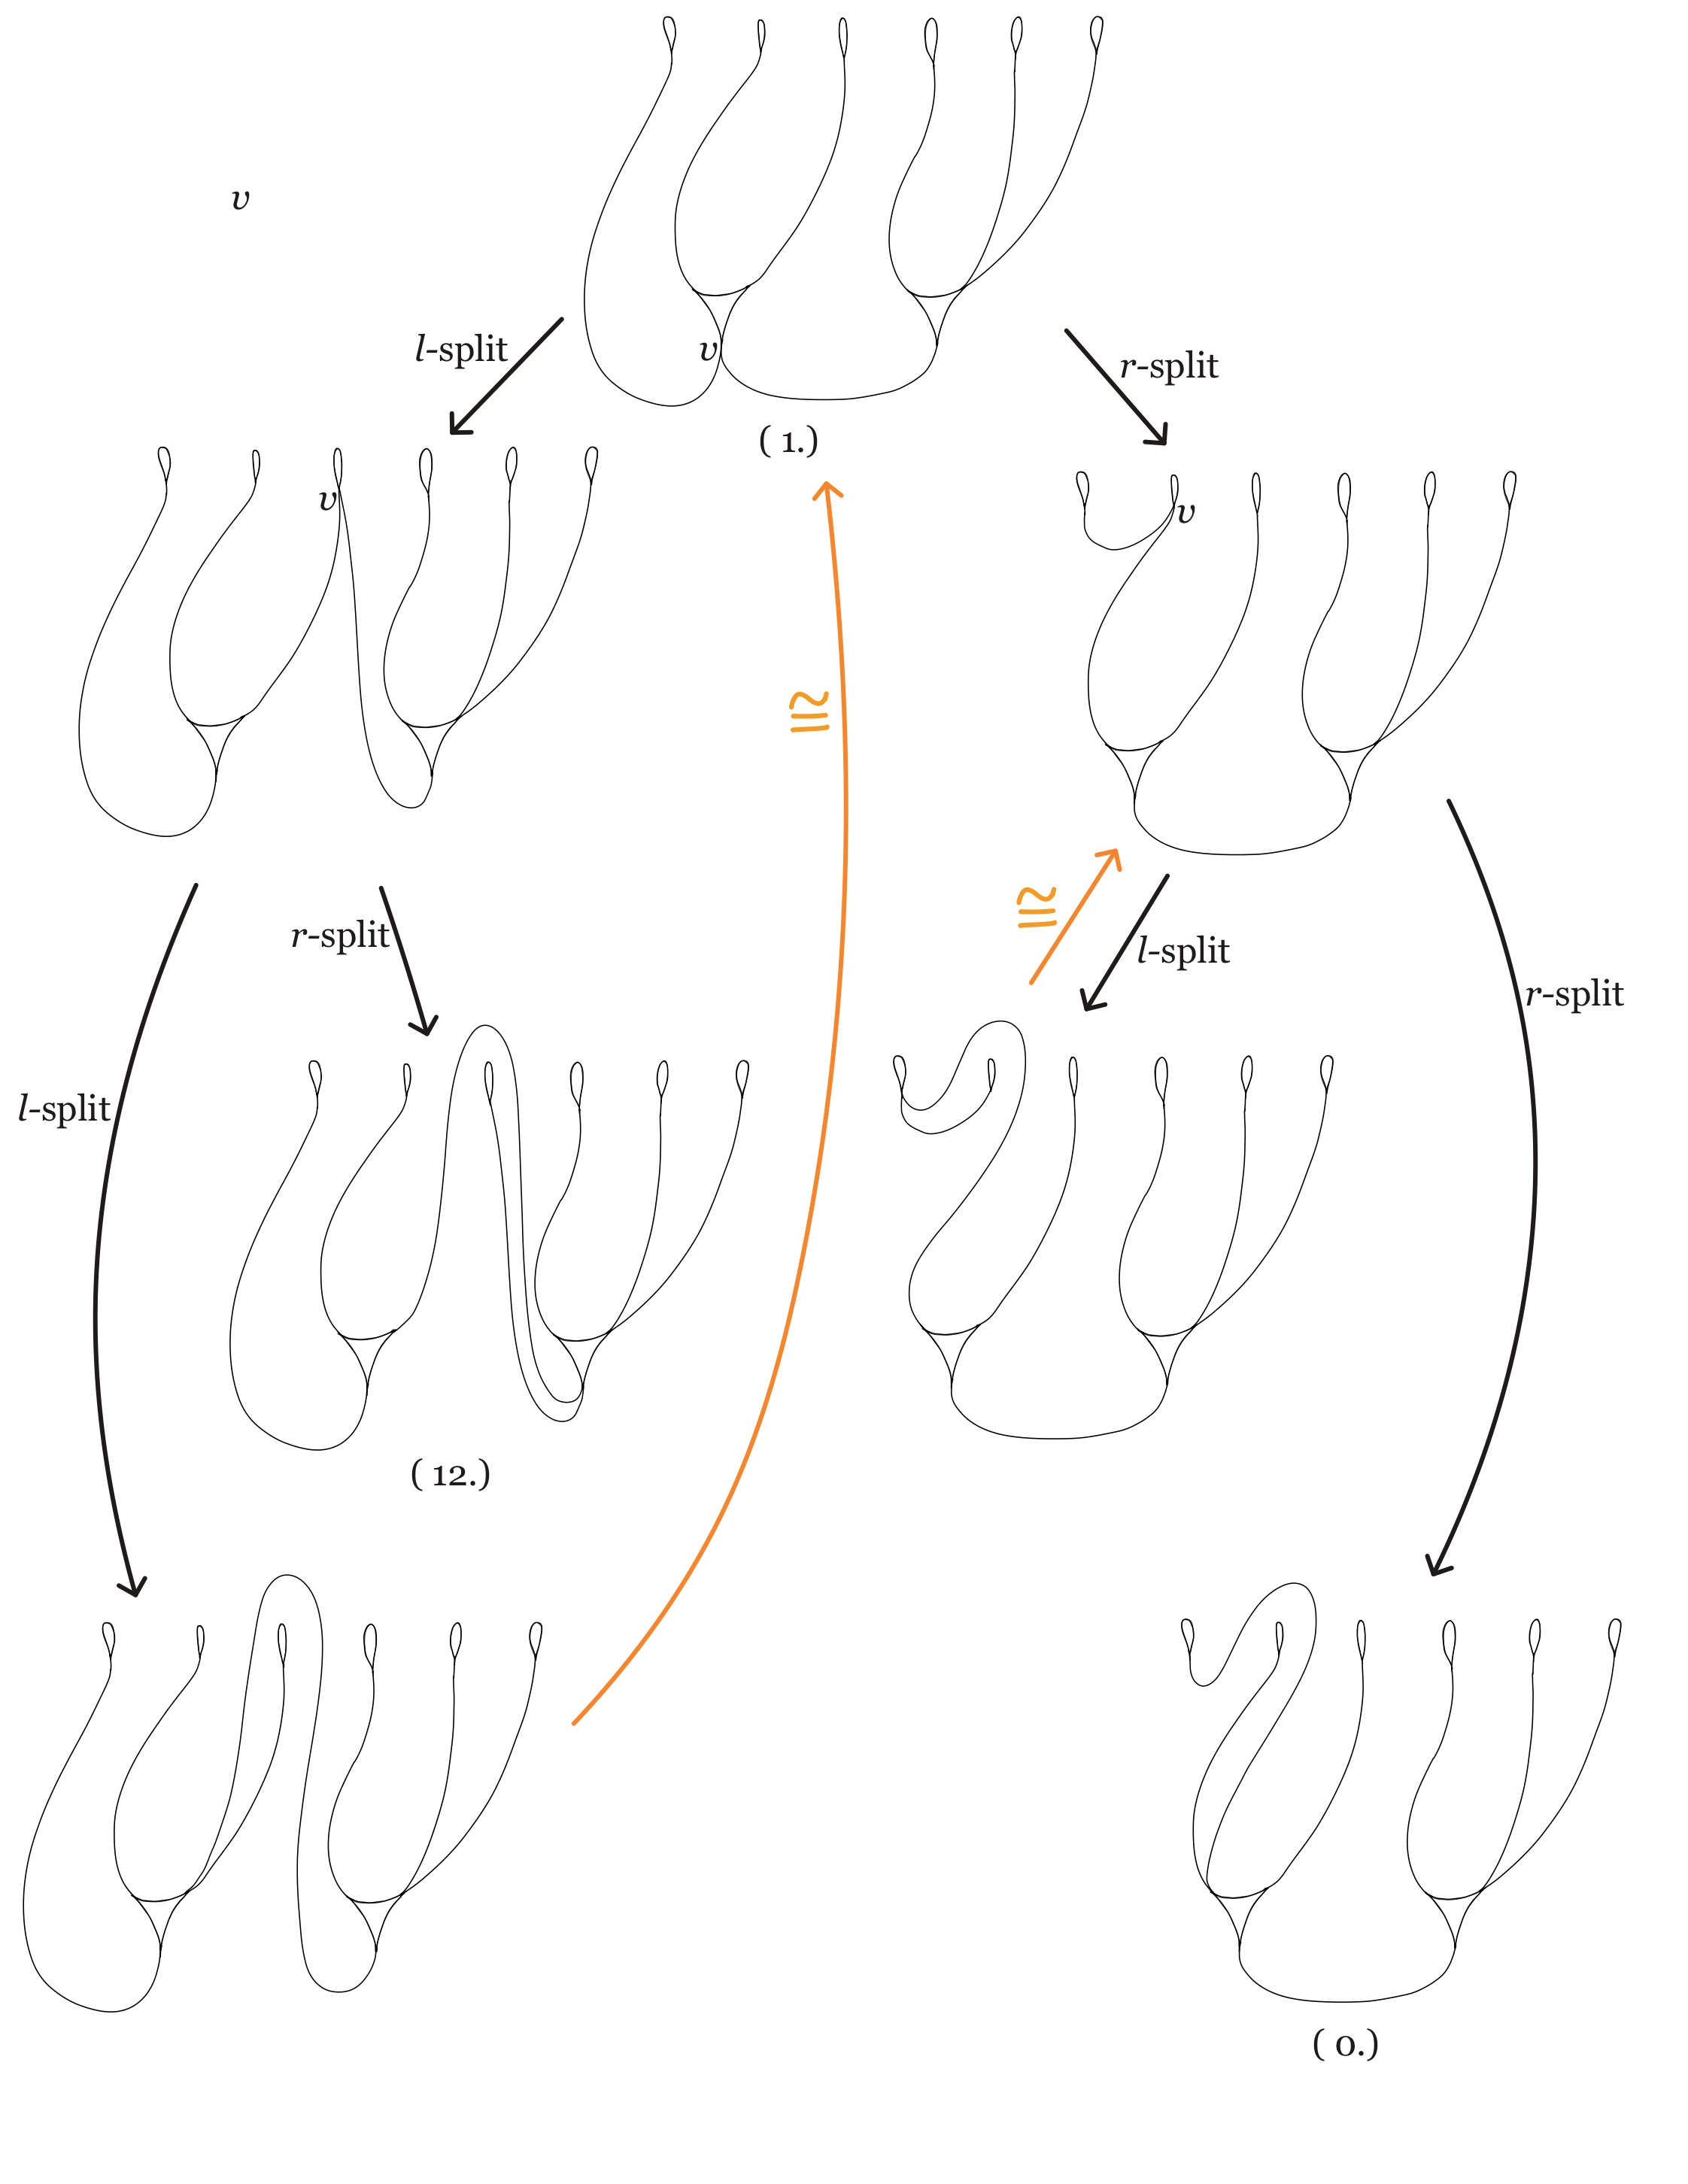
\includegraphics[width=\textwidth]{figures_splitting/1 Splitting-2.jpg}
%   The filename "1 Splitting-2.jpg" contains a space and starts with a
%   digit. While most modern LaTeX engines handle this via the graphicx
%   package, it is brittle: pdflatex on some systems requires the filename
%   to be wrapped in braces or quoted, and TeX tools downstream may choke
%   on the space. Recommended action: rename the file in the repo to
%   something like "splitting_diagram_example.jpg" and update the
%   \includegraphics line. Defer until the figure inventory pass at the
%   end of the audit.


% From the chaps_stratum_candelabra.tex audit:

% - FRAMING NOTE: The four-case split (Cases A, B, C, D) in the
%   "Path Notation and The Two Triangles" subsection distinguishes:
%     A: triangles fixed downstairs (lifts swapped upstairs)
%     B: triangles swapped, both lifts to same side
%     C, D: triangles swapped, mixed sides
%   Cases B, C, D all impose the same parity constraint (odd parity at
%   d-crossings); the only one with a different constraint is A (even
%   parity). The chapter is honest about this overlap, but if the
%   geometric distinction between B vs C/D never actually appears in
%   the per-track appendices, consider collapsing the four-case framing
%   to two cases (A vs B/C/D combined) to simplify the chapter
%   exposition. Verify against the appendices before making this change.

% - ADDITIONAL POSSIBLE BIB ENTRIES NEEDED for cross-reference targets
%   used in this chapter but not verified during the audit:
%     - cor:induce_by_braid_fulltwist (referenced at line 353 and 361)
%       — verify this corollary exists and has the correct label in
%       another chapter (likely chaps_stratum_candelabra's preliminaries
%       or chap_preliminaries).
%     - The labels chap:train tracks (referenced at line 30 of this
%       chapter) — this is the chaptraintracks.tex label with a space.
%       Confirmed in earlier audit notes that the actual label in
%       chaptraintracks.tex is "chap:train tracks" (with space). The
%       space in the label works in LaTeX but is unusual.


% From the chapsatellite.tex audit:

% - SECTION REMOVED: The original chapter included a final section
%   "Eliminating the (2,1)-Cable as a Candidate" (formerly
%   \label{sec:2_1_cable_candidate}). This section was redundant:
%   Lemma \ref{lem:satellite_trefoils_windingnumber_1} already excludes
%   the (2,1)-cable because (a) its winding number is 2, not 1, and
%   (b) its pattern P(U) = T_{2,1} is the unknot, not a trefoil. The
%   section has been replaced by a short forward-pointing remark to
%   Chapter \ref{chap:cable_detection}.

% - LABEL SPELLING: chap_preliminaries.tex line 151 defines
%     \label{theorem:nielsen-thruston classification}
%   with "thruston" misspelled (should be "thurston") and a space in
%   the label. The cross-reference from chapsatellite.tex line 117
%   uses the same misspelled key, so the reference works, but the
%   label is misspelled. Plan: at end-of-audit normalization pass,
%   correct the label to theorem:nielsen-thurston-classification
%   (no space, correct spelling), and update all references.

% - LABEL CONVENTION: Other labels with spaces in chap_preliminaries
%   confirmed to share this pattern:
%     theorem:thurston classification of knots (line 167)
%   These all work but should be normalized to underscored or
%   hyphenated forms at the end-of-audit normalization pass.

% - SEPARATING-CURVES CITATION FIX: At line 165 in the proof of
%   Lemma \ref{lem:satellite_CaseACaseB}, the original citation
%   \sidecite{baldwin2025lspaces} for the statement "every curve in
%   the canonical reducing system of a fibered knot in an L-space is
%   separating" was incorrect: this result is NOT in arXiv:2501.00914
%   ("L-spaces and knot traces", Baldwin-Sivek, Jan 2025). Verified by
%   reading the full paper. The cited paper does contain Proposition 2.3
%   (your \ref{prop:knottracesprop}, periodic outer map classification)
%   and the Nielsen-Thurston setup, but not the separating-curves fact.
%
%   The separating-curves result is from a forthcoming Baldwin-Sivek
%   paper, currently in preparation. The bib key has been changed to
%   \sidecite{BaldwinSivekInPrep}. A suggested bib entry:
%
%     @unpublished{BaldwinSivekInPrep,
%       author = {Baldwin, John A. and Sivek, Steven},
%       title  = {[forthcoming title]},
%       note   = {In preparation},
%       year   = {2026}
%     }
%
%   When the paper is posted/published, update this bib entry and key
%   accordingly. If the paper is not posted by submission time, the
%   "in preparation" form is acceptable; alternative form is "private
%   communication" attributed to John Baldwin.

% - BIB KEY VERIFICATION NEEDED for chapsatellite.tex:
%     - BZ03 (Burde-Zieschang, line 78): needs to exist in
%       bibliography.bib. The citation cites
%       "Corollary 4.15, Proposition 5.5" which strongly suggests
%       the standard reference: Burde and Zieschang, "Knots", de Gruyter
%       Studies in Mathematics 5, 2nd edition, 2003.
%     - schubert1953knoten (line 43, 46): Schubert's 1953 paper
%       "Knoten und Vollringe", Acta Math 90.
%     - HirasawaMurasugiSilver2008 (lines 94, 114): Hirasawa-Murasugi-Silver
%       "When does a satellite knot fiber?" Hiroshima Math J 38 (2008).
%     - baldwin2025lspaces (lines 138, 165, 198): Baldwin-Sivek,
%       "L-spaces and knot traces" or similar. Note: previous audit notes
%       flag that uniqueness and reduction results were re-attributed
%       to Baldwin-Sivek 2024; verify this is the same paper.
%     - birman1983abelian (line 129): Birman-Lubotzky-McCarthy, "Abelian
%       and solvable subgroups of the mapping class groups", Duke Math J
%       50 (1983).
%     - farb2012primer (line 283): Farb-Margalit, "A Primer on Mapping
%       Class Groups", available in /mnt/project/.
%     - hedden2018floer (line 325): Hedden-Mark, "Floer homology and
%       fractional Dehn twists", Adv. Math 324 (2018).
%     - honda2007right (line 370): Honda-Kazez-Matic, "Right-veering
%       diffeomorphisms of compact surfaces with boundary", Invent. Math
%       169 (2007).
%     - ozsvath2004holomorphic (line 360): Ozsvath-Szabo, "Holomorphic
%       disks and three-manifold invariants: properties and applications",
%       Ann. Math 159 (2004).
%     - Thurston1988 (line 121): Thurston's 1988 BAMS paper "On the
%       geometry and dynamics of diffeomorphisms of surfaces", or
%       Thurston's "Three-dimensional manifolds, Kleinian groups, and
%       hyperbolic geometry" BAMS 1982. The context (Nielsen-Thurston
%       classification with reducing systems) suggests the 1988 paper.


% From the chap_cable.tex audit:

% - HFK FIGURE ADDED: A bigraded HFK figure for C_{2,1}(T_{2,3}) has
%   been added, modeled after the granny HFK figure in chap_preliminaries
%   (\ref{fig:hfk_granny}). The rank table was computed via SnapPy's
%   knot_floer_homology(prime=2) function, which calls Szabo's HFK
%   computation library. Verified against:
%     - Symmetrization (A and -A have equal ranks),
%     - Alexander polynomial via Euler characteristic = t^2 - 1 + t^{-2},
%     - tau = 2 matching Hom's cabling formula for L-space companions,
%     - genus = 2 (top Alexander grading rank = 1),
%     - NOT thin: 7 generators split between diagonals delta = 1 (two
%       generators) and delta = 2 (five generators),
%     - NOT L-space: rank 2 in gradings A = +-1, exceeding L-space bound.
%   Code (for reproducibility):
%
%     import snappy
%     phi = [2, 1, 3, 2]   # Phi_2(sigma_1)
%     def cable_2q_seifert(beta, q, w):
%         word = []
%         for g in beta:
%             word += phi if g > 0 else [-x for x in reversed(phi)]
%         extra = q - 2*w
%         word += [1]*extra if extra > 0 else [-1]*(-extra)
%         return word
%     L = snappy.Link(braid_closure=cable_2q_seifert([1,1,1], q=1, w=3))
%     print(L.knot_floer_homology(prime=2)['ranks'])
%
%   The figure includes a citation to Szabo's HFK calculator under bib
%   key szabo2017knotfloercalculator (placeholder). The correct bib
%   reference may be Szabo's webpage or the embedded SnapPy library
%   citation; verify before submission.

% - BIB KEY: BaldwinSivek2022 -> BaldwinSivek2024. The original chapter
%   cited the almost-L-space-knot result via BaldwinSivek2022; this has
%   been updated to BaldwinSivek2024 for consistency with the rest of
%   the dissertation (the canonical reference for "almost L-space knot"
%   is Baldwin-Sivek 2024, as confirmed by reading their 2025 follow-up
%   "L-spaces and knot traces" which cites BS24a for the definition).

% - PROOF CLEANUP: lem:cable_satellite_classification (Lemma 11.X)
%   originally invoked an "infinite regress" argument that did not
%   close cleanly. The proof has been rewritten to use the explicit
%   three-case decomposition based on the factorization
%       Delta_K = Delta_{P(U)} * Delta_C(t^w)
%   in the variables |w|, g(C), and deg Delta_{P(U)}. Case 1
%   (|w|=2, g(C)=1, P(U)=unknot) gives the cable; Case 2
%   (|w|=1, g(C)=2, P(U)=unknot) is excluded by Hirasawa-Murasugi-Silver;
%   Case 3 (|w|=1, g(C)=1, deg Delta_{P(U)}=1) is excluded by an integer
%   coefficient check.

% - FIXED-POINT LEMMA REFERENCE: the chapter originally invoked
%   \ref{lemma:original monodromy has one fixed point} directly. That
%   lemma in chap_preliminaries is stated specifically for the granny
%   target. The argument has been inlined for the cable target, citing
%   Theorem theorem:ni-fibered (Ni-Ghiggini-Spano) for the rank-2
%   upper bound and farber2024fixed (Farber-Reinoso-Wang) for the
%   non-zero conclusion (the only FPF case is T_{2,5}, whose Alexander
%   polynomial differs from the cable's).
%   Alternative: Generalize lemma:original_monodromy_has_one_fixed_point
%   in chap_preliminaries to cover any genus-2 fibered knot with
%   rank-2 in next-to-top Alexander grading, then cite uniformly from
%   both chap_proof_of_main_theorem and chap_cable. Defer this
%   generalization decision.

% - VERIFY: count of 83 candidate braid families. The chapter states
%   "the same finite list of 83 candidate braid families (across the
%   Candelabra and the five surviving two-triangle tracks)". Verify
%   34 (Candelabra) + 49 (across Tracks 0, 1, 8, 13, 17) = 83 by
%   counting in the per-track appendices.

% - BIB KEYS TO VERIFY:
%   - petkova2013cables (originally on line 49, removed in this edit;
%     no longer cited in chap_cable but may be cited elsewhere).
%   - HeddenCableLSpace (newly introduced in the satellite-case proof;
%     the canonical reference is Hedden, "On knot Floer homology and
%     cabling II", IMRN 2009 or Trans. AMS 2009).
%   - szabo2017knotfloercalculator (newly introduced for the HFK figure;
%     verify the canonical reference for Szabo's HFK library).


% =====================================================================
% END OF NOTES
% =====================================================================
